  \mysection{The Mystic}{trope-mystic}

  \flavor{Creedsmen roll out across the dying dawn - Sacred Israel holy mountain Zion - Sun beams down on to the sandsea reigns - Caravan migrates through deep sandscape - Lungsmen unearth the creed of Hasheeshian - Procession of the weed-priests to cross the sands - Desert legion smoke-covenant is complete - Herb bales re-tied on to backs of beasts - Arise arise arise - The Son of the God of Israel - Jordan river flows on evermore - Bathe in glow of sunlight's beating rays - They feel the serpent's standard rule our day \Tilde Sleep, "Dopesmoker"}


\begin{center}
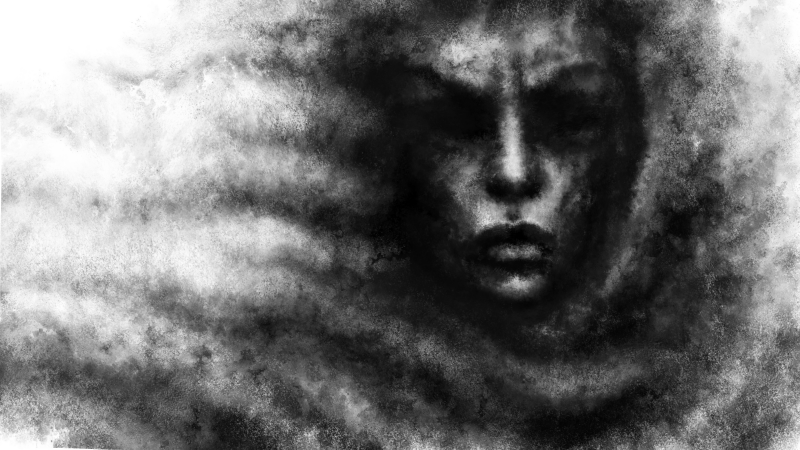
\includegraphics[width=\linewidth,keepaspectratio=true]{tropes/MysticHeader}
\end{center}


 \mysubsection{Creation}{mystic-creation}

  Write down the following information on your \mylink{Adventurer Sheet}{adventurer-sheet.4}
  
  \callout {
    \mybullet {
        \item You start with \mybold{6 Flesh and 4 Grit}.
        \item Move your \FOC~ \DCUP (to a d10). Pick \VIG, \DEX, or \INT and move it \DCDOWN (to a d6).
        \item If you need to \RSTRY{\FOC}, you only fail on a natural 1 (instead of a 1 or 2). Put a check next to \FOC on your Adventurer Sheet so you don't forget.
        \item Choose three different \mylink{Virtues}{mystic-virtues} and one \mylink{Complication}{mystic-complications}. Modify your sheet as necessary.
        \item Write down your \mylink{Starting Gear}{mystic-starting-gear}.
    }
 }


\newpage
\begin{multicols*}{2}\raggedcolumns

  \myhighlight{Mortal}{mystic-mortal}
    
  You are a creature of Order, and possess a soul - and are thus \mybold{Hallowed}.


\mysubsection{Starting Mystic Virtues}{mystic-virtues}

    \begin{center}
        \myemph{Choose 3 of the following}
    \end{center}

  

    \myhighlight{Bruja}{mystic-virtue-bruja} 

    You gain a \UDD{d4} of \mylink{Juju}{cruces-mojo} that you may use to perform \mypg{Arcana: Witchcraft}{arcana-witchcraft}. See the section on the \mypg{Crux of Mojo}{cruces-mojo}.

   
    \myhighlight{Charms}{mystic-virtue-vulgate-charms}

    You can perform the \mypg{Vulgate of Charms}{vulgate-charms} at will.


    \myhighlight{Cunning Folk}{mystic-virtue-cunning-folk}


    \mybullet{
        \item Gain 1 \mylink{Cunning Pip}{cunning-pips} (this is in addition to the Cunning Pip you would gain through \mylink{Virtue: Mombo}{mystic-virtue-mombo}). See the section on \mypg{Cunning}{cunning} for more info.
        \item You gain a \mylink{Familiar}{occultism-bind-familiar} without needing to go through the occult ritual. See \mylink{Bind Familiar}{occultism-bind-familiar} under the \mypg{Occultism}{cunning-occultism} section for details about what your familiar can do.
    }

\begin{center}
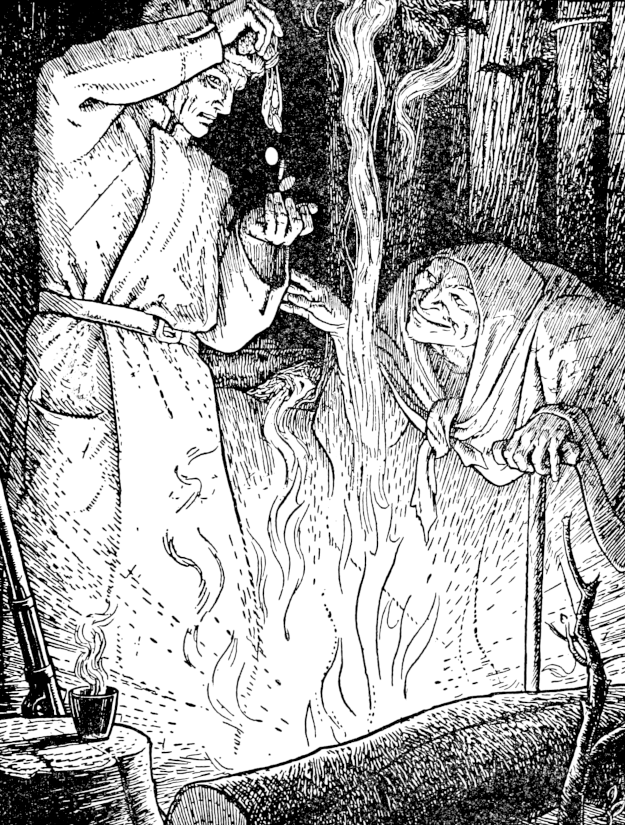
\includegraphics{tropes/WitchCoins}
\end{center}



    \myhighlight{Hand of God}{mystic-virtue-hand-of-god}

    \mybullet {
        \item You have \mybold{Found Religion}; choose a \mybold{Paradigm} and name the \mybold{Small God} that is the object of your worship. See the section on the \mypg{Crux of Faith}{cruces-faith}.
        \item You gain a single \mybold{Faith Die}; this Faith Die is in addition to any other Faith Dice you may acquire through \mylink{Initiate}{mystic-virtue-initiate} or \mylink{Miracle Worker}{mystic-virtue-miracle-worker}. Your \MAX Faith is 3. 
        \item You may roll a single Faith Die and add its result to \mybold{any} of your \RO or \RB tries. You may roll this Faith Die \myital{after} you roll your try (it doesn't have to be at the same time), but you can only roll one Faith Die per try.
    }


    \myhighlight{Holy Warrior}{mystic-virtue-holy-warrior}

    \mybullet {
        \item You may wield any weapon using your \FOC (instead of \VIG, \DEX, or \INT).
        \item You gain +4 \MAX \mylink{Grit}{adventurer-flesh-grit}.
    }



    \myhighlight{Initiate}{mystic-virtue-initiate}

    \mybullet {
        \item You have \mybold{Found Religion}; choose a \mybold{Paradigm} and name the \mybold{Small God} that is the object of your worship. See the section on the \mypg{Crux of Faith}{cruces-faith}.
        \item You gain a single \mybold{Faith Die}; this Faith Die is in addition to any other Faith Dice you may acquire through \mylink{Hand of God}{mystic-virtue-hand-of-god} or \mylink{Miracle Worker}{mystic-virtue-miracle-worker}. Your \MAX Faith is 5. 
        \item You gain a holy symbol - a minor \mypg{Holy Relic}{miracle-holy-relic} that contains 1 Faith die. This holy symbol is necessary for performing your \mylink{Liturgies}{arcana-liturgies}.
        \item You learn the Liturgy of the Novitiates of your Small God. See the section on \mypg{Liturgies}{arcana-liturgies} and choose which two Hymns, Orisons, Lorespells, or Ablutions you know.

}

\newpage

    \myhighlight{Itinerant}{mystic-virtue-itinerant}

    You are no stranger to the trials and travails of life; you have accumulated some gear on your journeys. You can pick \mybold{three} of the following:

    \callout {
      \footnotesize {
      \mybullet {
        \item a suit of \mylink{Light Armor}{gear-armor};
        \item a suit of \mylink{Medium Armor}{gear-armor};
        \item a Magical athame (treat as a \mylink{Dagger}{gear-dex-weapons} that can strike Monsters only affected by magic);
        \item a \mylink{Quarterstaff}{gear-int-weapons};
        \item a \mylink{Crossbow}{gear-foc-weapons} and a \mylink{Quiver of Bolts}{gear-equipment};
        \item 5 picks from the \mylink{Tools}{gear-equipment} table;
        \item a pouch of 3 gems (roll on the \mylink{Gems table}{appendix-a-gems} in Appendix A);
        \item \UDD{d4} of 3 different \mylink{Narcotics}{gear-narcotics}, or \UDD{d10} of one;
        \item a \mylink{Mule}{gear-transport};
      }
      }
    }


    \myhighlight{Medicine}{mystic-virtue-vulgate-medicine}

    You can perform the \mypg{Vulgate of Medicine}{vulgate-medicine} during \mypg{Downtime}{downtime-shopping}.

    \myhighlight{Miracle Worker}{mystic-virtue-miracle-worker}

    \mybullet {
        \item You have \mybold{Found Religion}; choose a \mybold{Paradigm} and name the \mybold{Small God} that is the object of your worship. See the section on the \mypg{Crux of Faith}{cruces-faith}.
        \item You gain a single \mybold{Faith Die}; this Faith Die is in addition to any other Faith Dice you may acquire through \mylink{Hand of God}{mystic-virtue-hand-of-god} or \mylink{Initiate}{mystic-virtue-initiate}. Your \MAX Faith is 4.
        \item You may perform \mylink{Miracles}{wonders-miracles} using your Faith Die. See the section on \mylink{Miracles}{wonders-miracles} under \mypg{Wonders}{wonders} for more information.
    }

    \cbreak
    
    \myhighlight{Mombo}{mystic-virtue-mombo}
  
    \mybullet {
        \item Gain 1 \mylink{Cunning Pip}{cunning-pips} (this is in addition to the Cunning Pip you would gain through \mylink{Virtue: Cunning Folk}{mystic-virtue-cunning-folk}).

         \item You may create \mylink{Marvels}{cunning-marvels} using your Cunning Pip(s). See the section on \mypg{Cunning}{cunning} for more info.
    }



    \myhighlight{Sacraments}{mystic-virtue-vulgate-sacraments}
   
    You gain a single Grace die (d4) which allows you to perform the \mypg{Vulgate of Sacraments}{vulgate-sacraments}.


    \myhighlight{Sacred Flesh}{mystic-virtue-sacred-flesh}

    Your flesh is blessed by the Small Gods or imbued with unholy power. Gain +2 \MAX \mylink{Flesh}{adventurer-flesh-grit}, and your \DEATH moves \DCUP to \mybold{Tough (d4)}. 


  \myimage{tropes/Mystic_1}

\newpage

\mysubsection{Mystic Complications}{mystic-complications}

    \begin{center}
        \myemph{Choose 1 of the following}
    \end{center}

  \myhighlight{Animal Lover}{mystic-animal-lover}

  You love all kinds of animals; you refuse to ride beasts of burden (including being pulled in a cart by them), eat meat, or suffer the mistreatment of an animal (does not apply to animals that are actively trying to kill you).

  \myhighlight{Burn the Witch!}{mystic-complication-witch}
  
  Any time you stay in a Tiny \mylink{Settlement}{civilization-settlements}, you run the risk of being accused of witchcraft. If you stay in a Tiny thorp, dorf, etc. roll 2d6 - on a 2 (snake-eyes) you're accosted for poisoning the well water / getting the farmer's daughter pregnant (your gender is irrelevant) / making the chickens sick, etc. If you roll a 12 (boxcars), you'll be called on to do something important - deliver a baby, heal someone's fever, etc.

  \myhighlight{Cat's Eyes}{mystic-cats-eyes}

  Through some mishap, you have the eyes of a cat. They unfortunately don't allow you to see very well in the dark (treat as if you were holding a candle, probably enough to read by but not much else). They glow in the dark, however, making it difficult (though creepy) to sneak up on the unwary.

  \myhighlight{Heretic}{mystic-complication-heretic}

  Name a Small God. This God is heretical to your belief; its followers must be slain, its temples desecrated, and its name forgotten.

\cbreak

  \myhighlight{Imma Smoke It}{mystic-imma-smoke-it}

  You're constantly looking for new and better ways to transcend the mortal plane and see into the heart of the universe, i.e. to get high. If there's a weird mushroom, you're going to try it. Some kind of slime, put it in your pipe and see what happens. I hope you've decided to bump your Toxins Save.

  \myhighlight{My Name is Earl}{mystic-name-is-earl}

  You have set out on the path of the Mystic thanks to the help and sacrifice of another. You can never repay this debt, so you must pay forward kindness whenever possible. Tell the Arbiter what this debt is, and who you owe it to.

  \myhighlight{Otherworldly}{mystic-otherworldly}

  You are eerie, uncanny, and unreal. You don't cast a reflection, your footprints appear backwards, etc. Common folk want nothing to do with you; more powerful persons you meet hold you at arm's length. Tell the Arbiter what your alien nature is reflected in your Adventurer.

  \myhighlight{Transubstantiation}{mystic-transubstantiation}

  You require your own flesh and blood to fuel your \mylink{Cunning}{cunning} and \mylink{Miracles}{wonders-miracles} - not a lot, anywhere between a few drops and a goblet-full; a small slice off a limb to a fingertip's worth. The effects of using your own flesh and blood in this way can have ... interesting effects ... at the complete discretion of the Arbiter.

  \myhighlight{The Unseelie}{mystic-unseelie}

  The Unseelie are Unhallowed, anathema in the eyes of \TheAuthority. The Unseelie deserve your contempt at best, to be burned at the stake at worst.

  Alternately, the Unseelie are cursed and alone. They deserve your pity and understanding, and to be protected from the infantile fears and hatreds of Mortals.

  \myhighlight{Vow of Poverty}{mystic-vow-of-poverty}

  You have taken a vow of poverty. You will never possess more money than you need to live a basic existence; you live as humbly as you possibly can. You still insist on your full share of treasure, but you will donate it or give it away. 


  \mysubsection{Starting Gear}{mystic-starting-gear}
    \callout {
              \footnotesize {

    In addition to any gear you might have gained from Virtues, you have:
    

      \mybullet {
        \item 2 iron pieces; 
        \item a \mylink{Quarterstaff}{gear-dex-weapons} or two iron \mylink{Daggers}{gear-dex-weapons};
        \item \UDD{d4} of \mylink{Personal Provisions}{gear-equipment};
        \item 3 picks OR 5 rolls on the \mylink{Random Items}{appendix-a-random-items} table in Appendix A
      }
    }
}

\myhighlight{What Next?}{mystic-what-next}

If you're playing a "cleric" type of Mystic, start with the \mypg{Crux of Faith}{cruces-faith}. Understand the powers of your Small God's \mypg{Paradigm}{faith-paradigm} and the \mypg{Arcana: Liturgies}{arcana-liturgies} you can perform. Finally, you may want to take a look at \mypg{Miracles}{wonders-miracles}, which are "powered" by your Faith.

\cbreak

\myimage{tropes/Mystic_3}

If you're playing a "witch" type of mystic, start with the \mypg{Crux of Mojo}{cruces-mojo}. Understand how your \mypg{Juju}{cruces-mojo-juju} works, and take a look at the \mypg{Arcana: Witchcraft}{arcana-witchcraft} you can perform. Finally, you may want to take a look at and understand \mypg{Cunning}{cunning}, and how you can perform \mypg{Marvels}{cunning-marvels} and/or \mypg{Occultism}{cunning-occultism} with Cunning Pips.

\end{multicols*}
